\chapter{Sprint 2 – User and Product Management (Admin)}

\section{Introduction}

The second sprint focused on building the administrative interface for user and product management. While Sprint 1 established secure authentication and role-based routing, Sprint 2 addressed the critical administrative functions that enable proper system operation: managing user accounts, product catalog maintenance, and inventory control.

This sprint was essential for establishing the foundation of the business logic, as administrators need comprehensive tools to maintain the system's data integrity and operational efficiency.

\section{Sprint 2 Backlog}

\begin{table}[H]
\centering
\begin{tabular}{|c|p{10cm}|c|}
\hline
\textbf{Task ID} & \textbf{Task Description} & \textbf{Status} \\
\hline
S2-T1 & Create admin dashboard layout & Completed \\
S2-T2 & Build user management interface & Completed \\
S2-T3 & Add product management features & Completed \\
S2-T4 & Implement inventory tracking & Completed \\
S2-T5 & Add form validation & Completed \\
S2-T6 & Test admin functions & Completed \\
\hline
\end{tabular}
\caption{Sprint 2 – Backlog and Implementation Plan}
\label{tab:sprint2-backlog}
\end{table}

\section{Functional Specification}

The admin interface was designed to provide comprehensive management capabilities for system administrators. The dashboard includes:

\begin{itemize}
  \item \textbf{User Management Module:} Create, read, update, and delete user accounts with role assignments
  \item \textbf{Product Management System:} Full CRUD operations for product catalog maintenance
  \item \textbf{Inventory Control:} Real-time stock level monitoring and adjustment capabilities
  \item \textbf{Role and Permission Management:} Assign and modify user roles (Admin, Cashier)
  \item \textbf{System Analytics Dashboard:} Overview of system health and usage statistics
\end{itemize}

Each module was designed with intuitive navigation and responsive layouts using Tailwind CSS components.

\section{Use Case Diagram}

\begin{figure}[H]
  \centering
  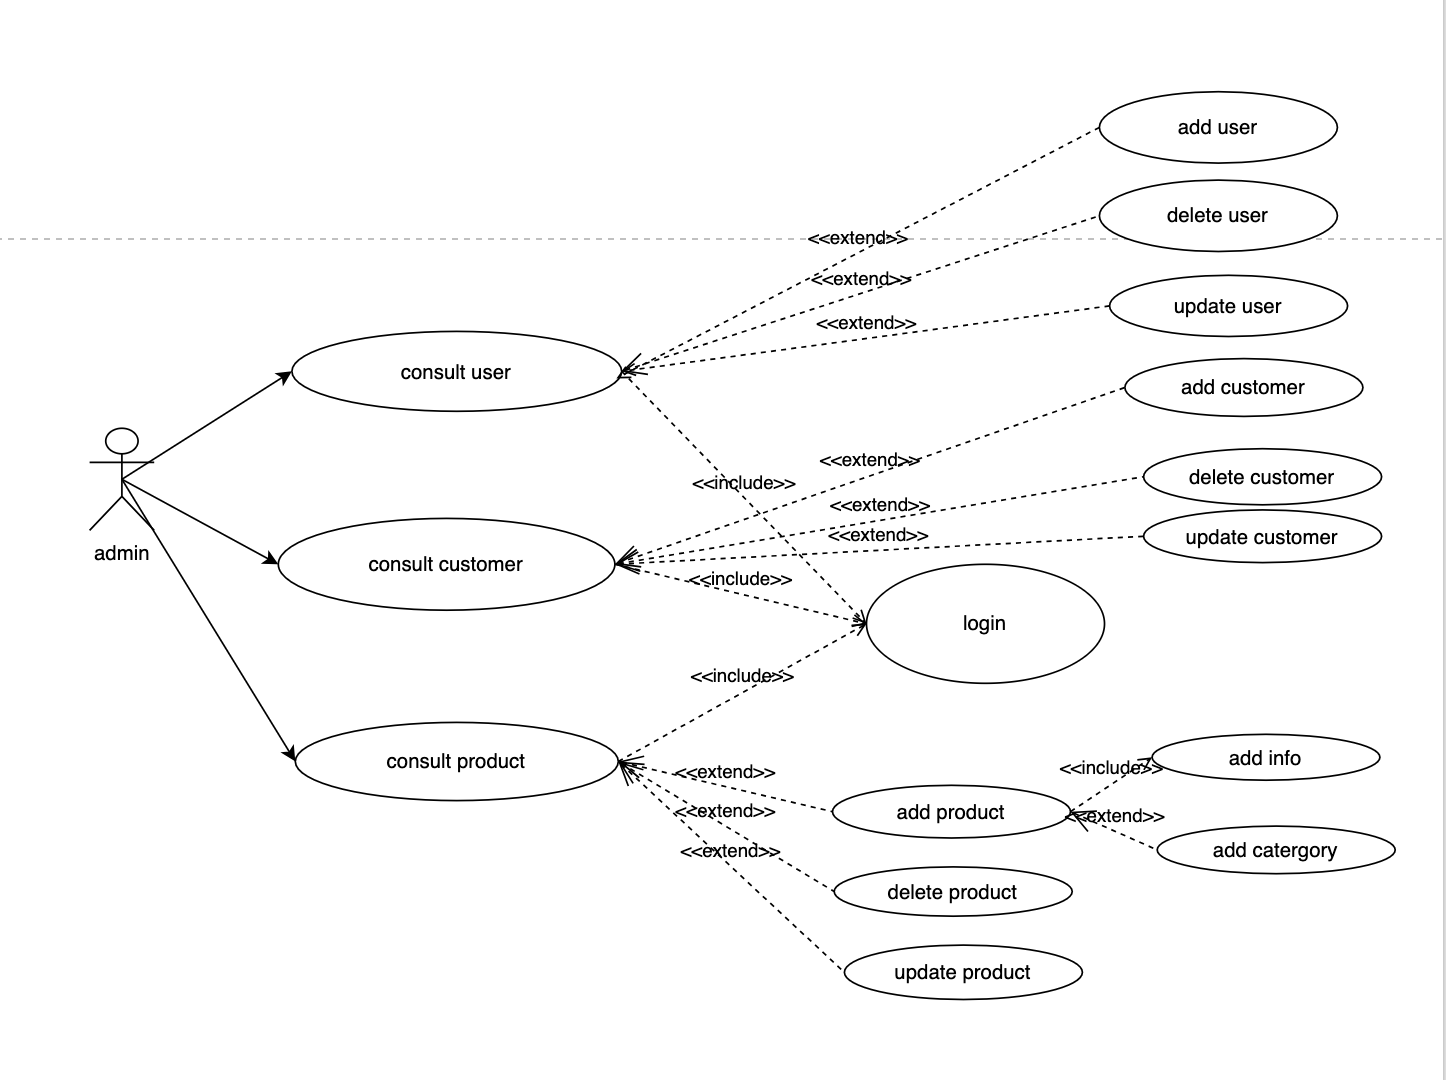
\includegraphics[width=0.9\textwidth]{figures/images/sprint2usecase.png}
  \caption{Sprint 2 – User and Product Management Use Case Diagram}
  \label{fig:sprint2-usecase}
\end{figure}

\section{User Management Implementation}

\subsection*{User Account Creation}

The user creation system allows administrators to:
\begin{itemize}
  \item Add new user accounts with email and initial password
  \item Assign appropriate roles (Admin or Cashier)
  \item Set user status (Active/Inactive)
  \item Configure user permissions and access levels
\end{itemize}

\subsection*{User Profile Management}

Existing user accounts can be managed through:
\begin{itemize}
  \item Profile editing (name, email, contact information)
  \item Role modification and permission updates
  \item Password reset functionality
  \item Account status management (activation/deactivation)
\end{itemize}

\section{Product Management System}

\subsection*{Product Catalog Operations}

The product management interface provides:
\begin{itemize}
  \item \textbf{Add New Products:} Name, description, price, category, and image upload
  \item \textbf{Edit Existing Products:} Modify product details and pricing
  \item \textbf{Product Categories:} Organize products into logical categories
  \item \textbf{Bulk Operations:} Import/export product data via CSV
\end{itemize}

\subsection*{Inventory Management}

Stock control features include:
\begin{itemize}
  \item Real-time stock level tracking
  \item Low stock alerts and notifications
  \item Manual stock adjustments (additions/deductions)
  \item Stock movement history and audit trail
\end{itemize}

\section{Database Schema for Admin Functions}

The database was extended to support administrative operations with the following key tables:

\begin{itemize}
  \item \textbf{users:} Stores user account information, roles, and permissions
  \item \textbf{products:} Complete product catalog with inventory data
  \item \textbf{categories:} Product categorization system
  \item \textbf{inventory\_movements:} Audit trail for stock changes
  \item \textbf{user\_sessions:} Track user activity and session management
\end{itemize}

\section{Class Diagram}

\begin{figure}[H]
  \centering
  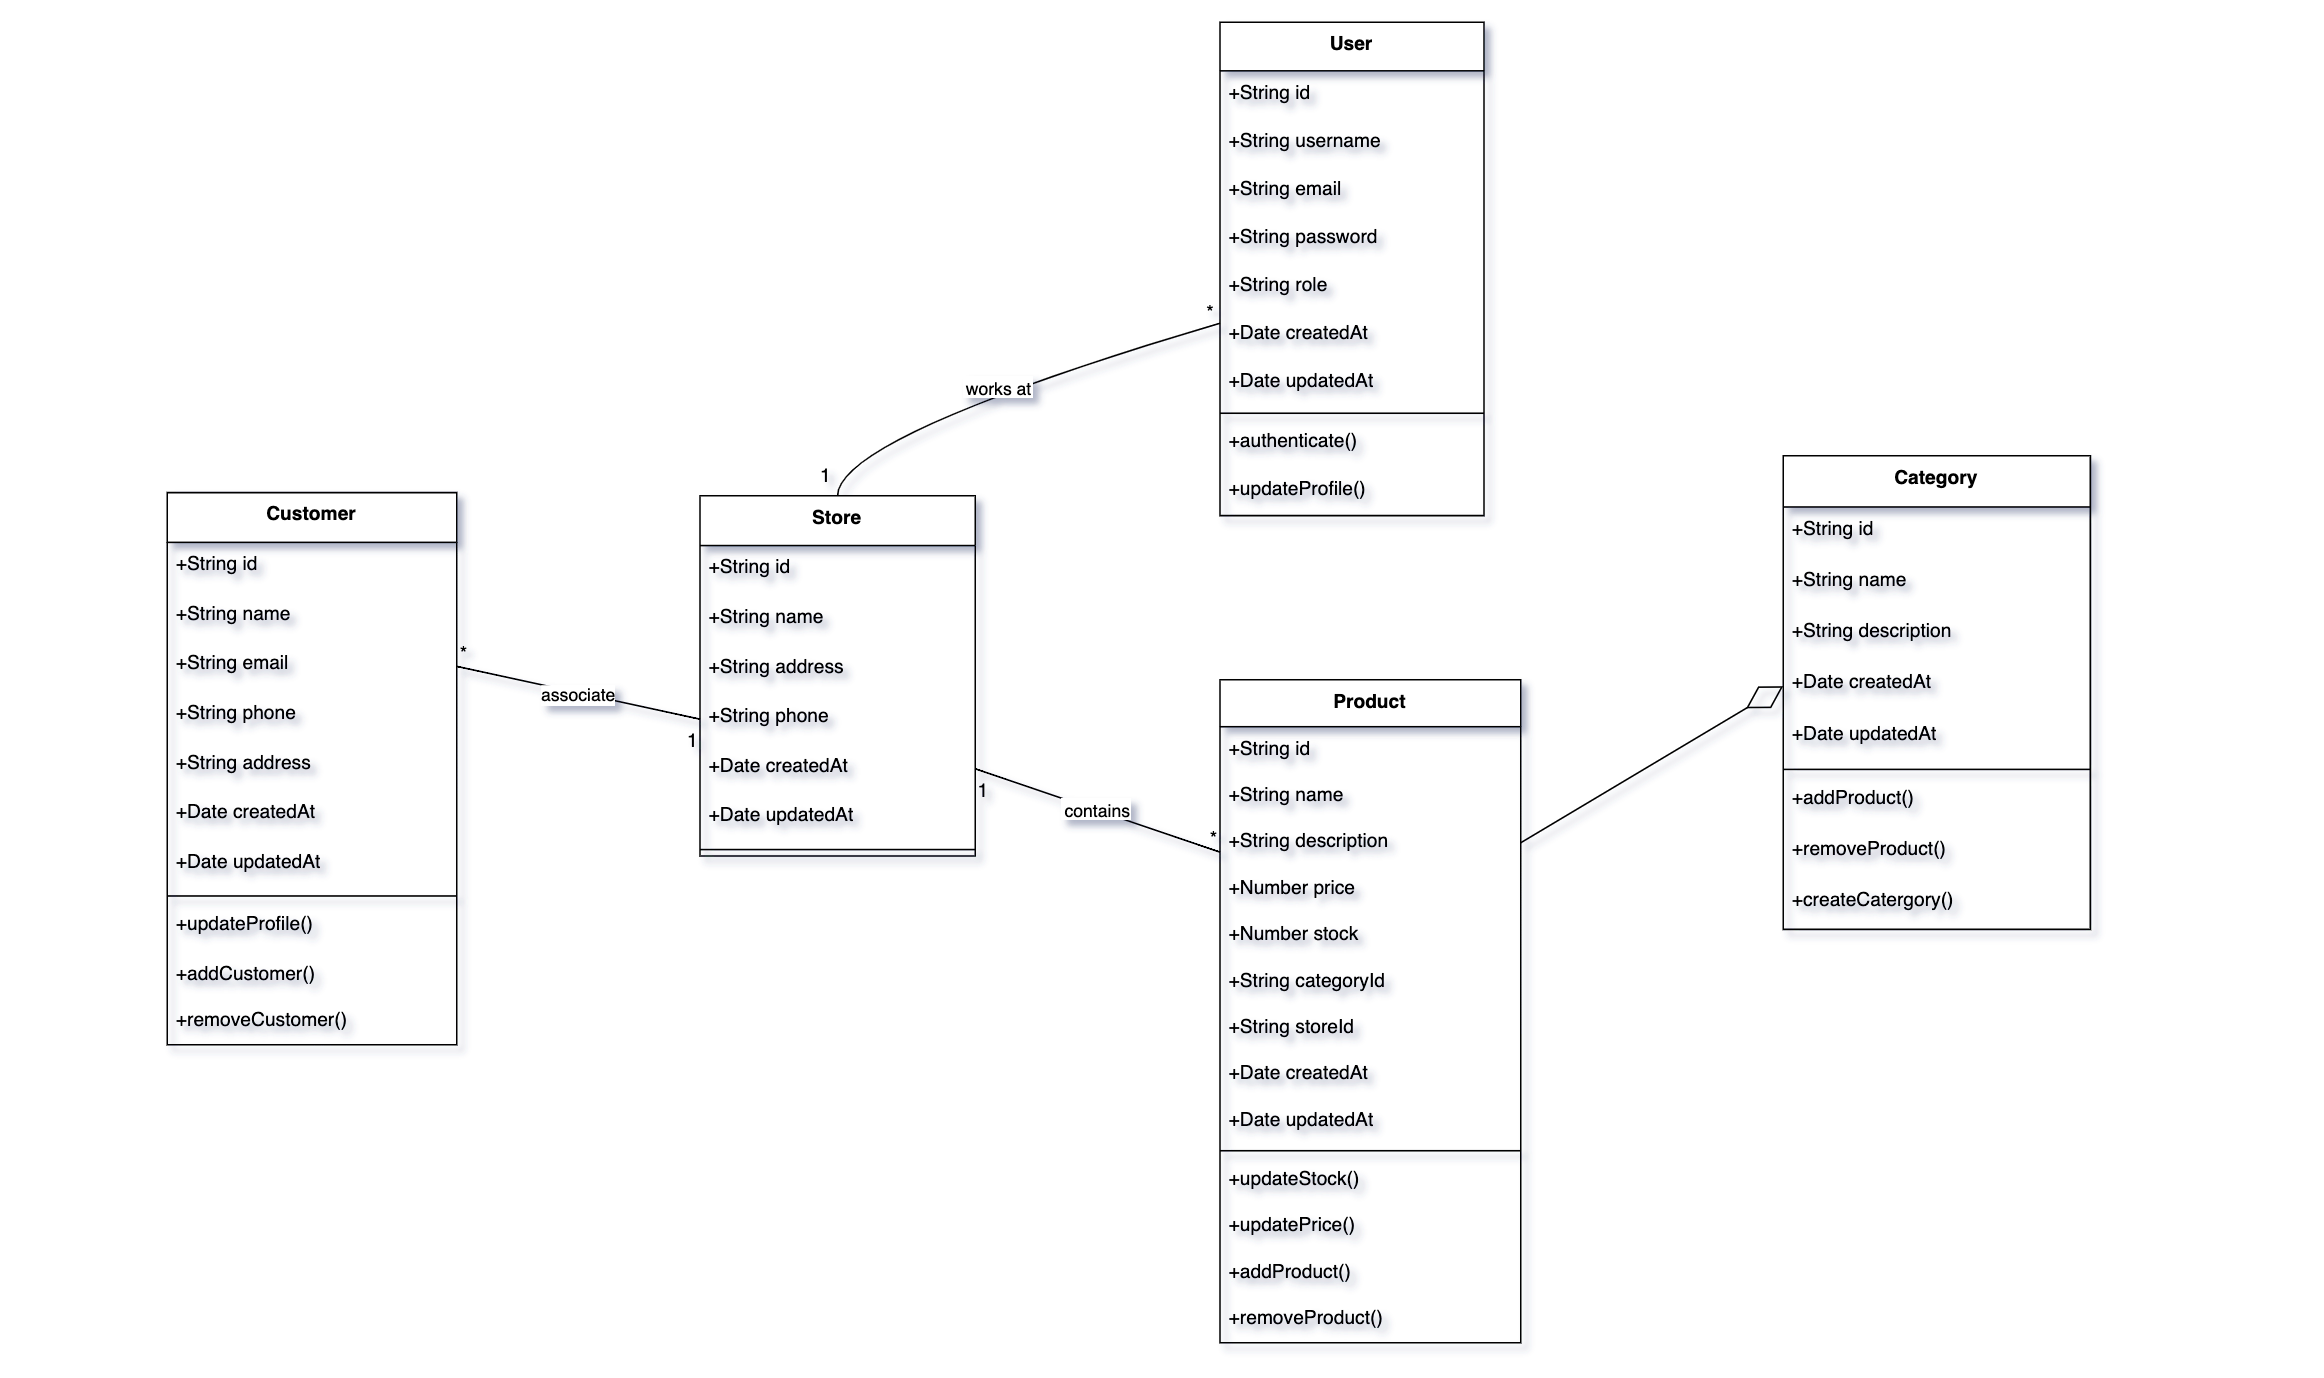
\includegraphics[width=0.9\textwidth]{figures/images/sprint2class.png}
  \caption{Sprint 2 – Admin Management Class Diagram}
  \label{fig:sprint2-class}
\end{figure}

\section{Sequence Diagrams}

\subsection{User Management Sequence}

\begin{figure}[H]
  \centering
  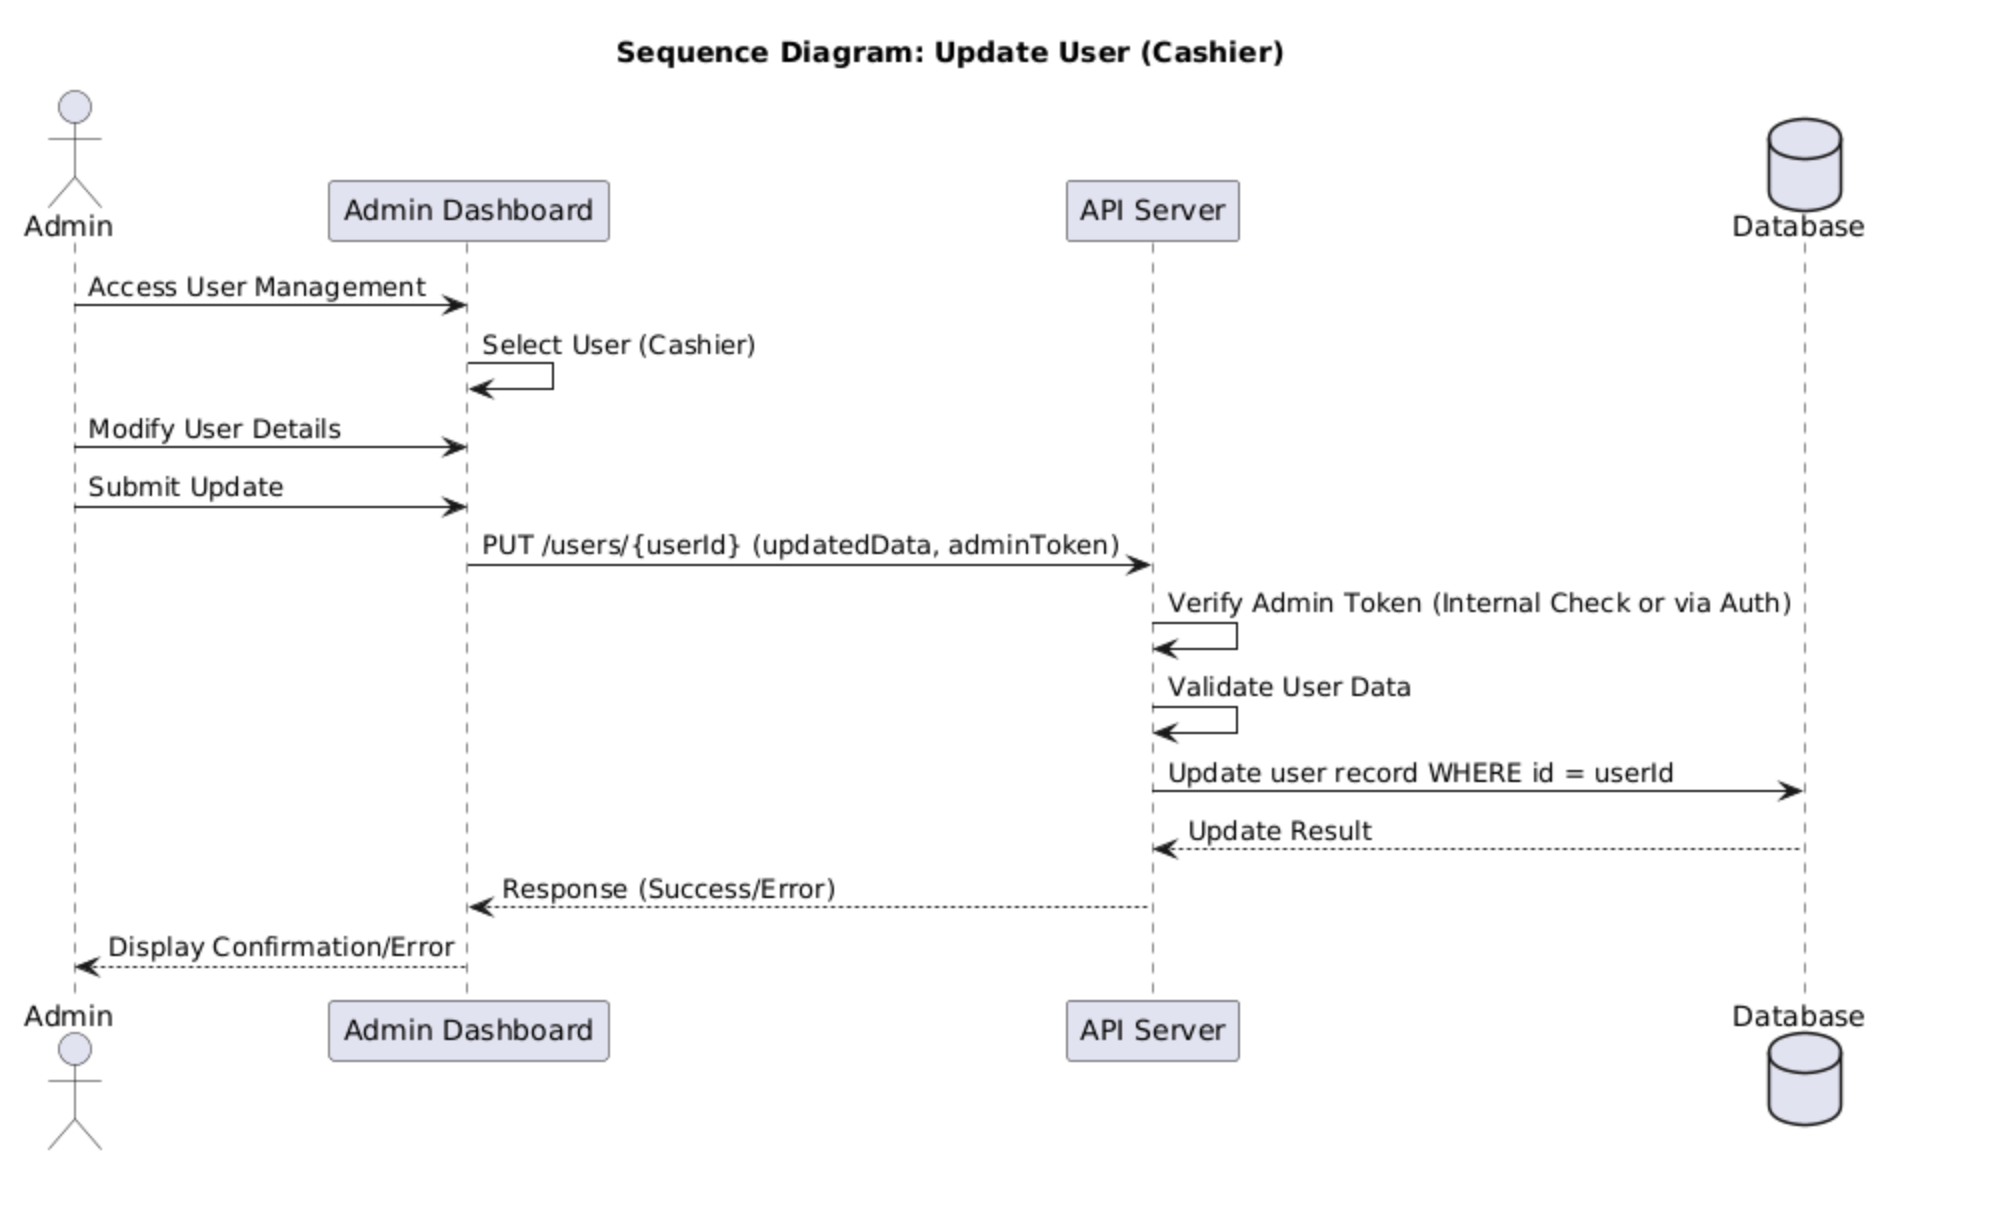
\includegraphics[width=0.9\textwidth]{figures/images/sprint2sequence diagram(update user).png}
  \caption{Sprint 2 – Update User Sequence Diagram}
  \label{fig:sprint2-update-user}
\end{figure}

\subsection{Customer Management Sequence}

\begin{figure}[H]
  \centering
  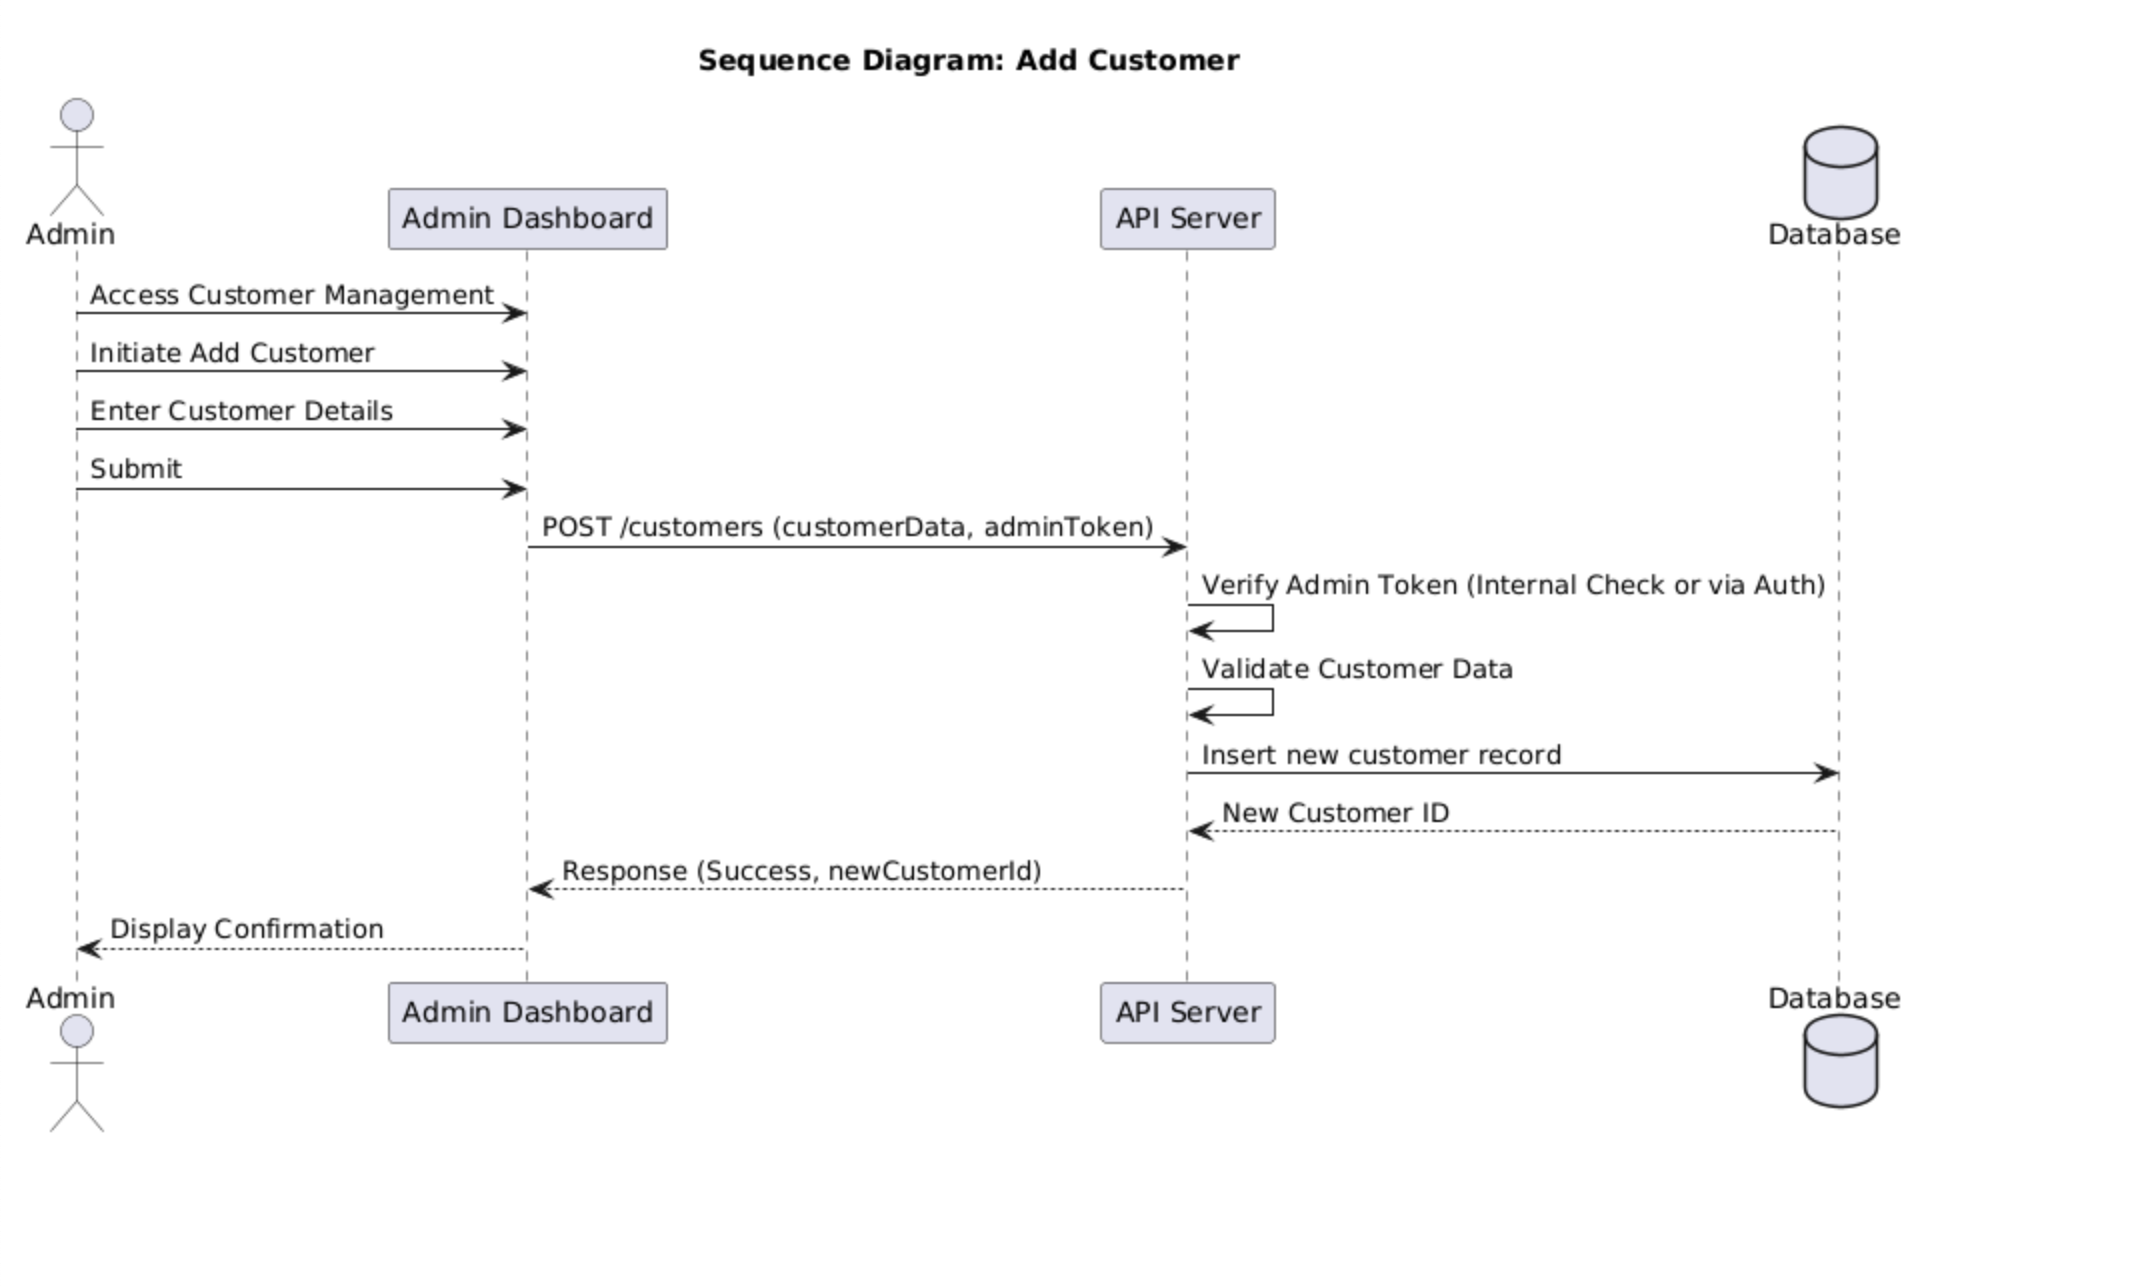
\includegraphics[width=0.9\textwidth]{figures/images/sprint2sequence(add customer).png}
  \caption{Sprint 2 – Add Customer Sequence Diagram}
  \label{fig:sprint2-add-customer}
\end{figure}

\subsection{Product Management Sequence}

\begin{figure}[H]
  \centering
  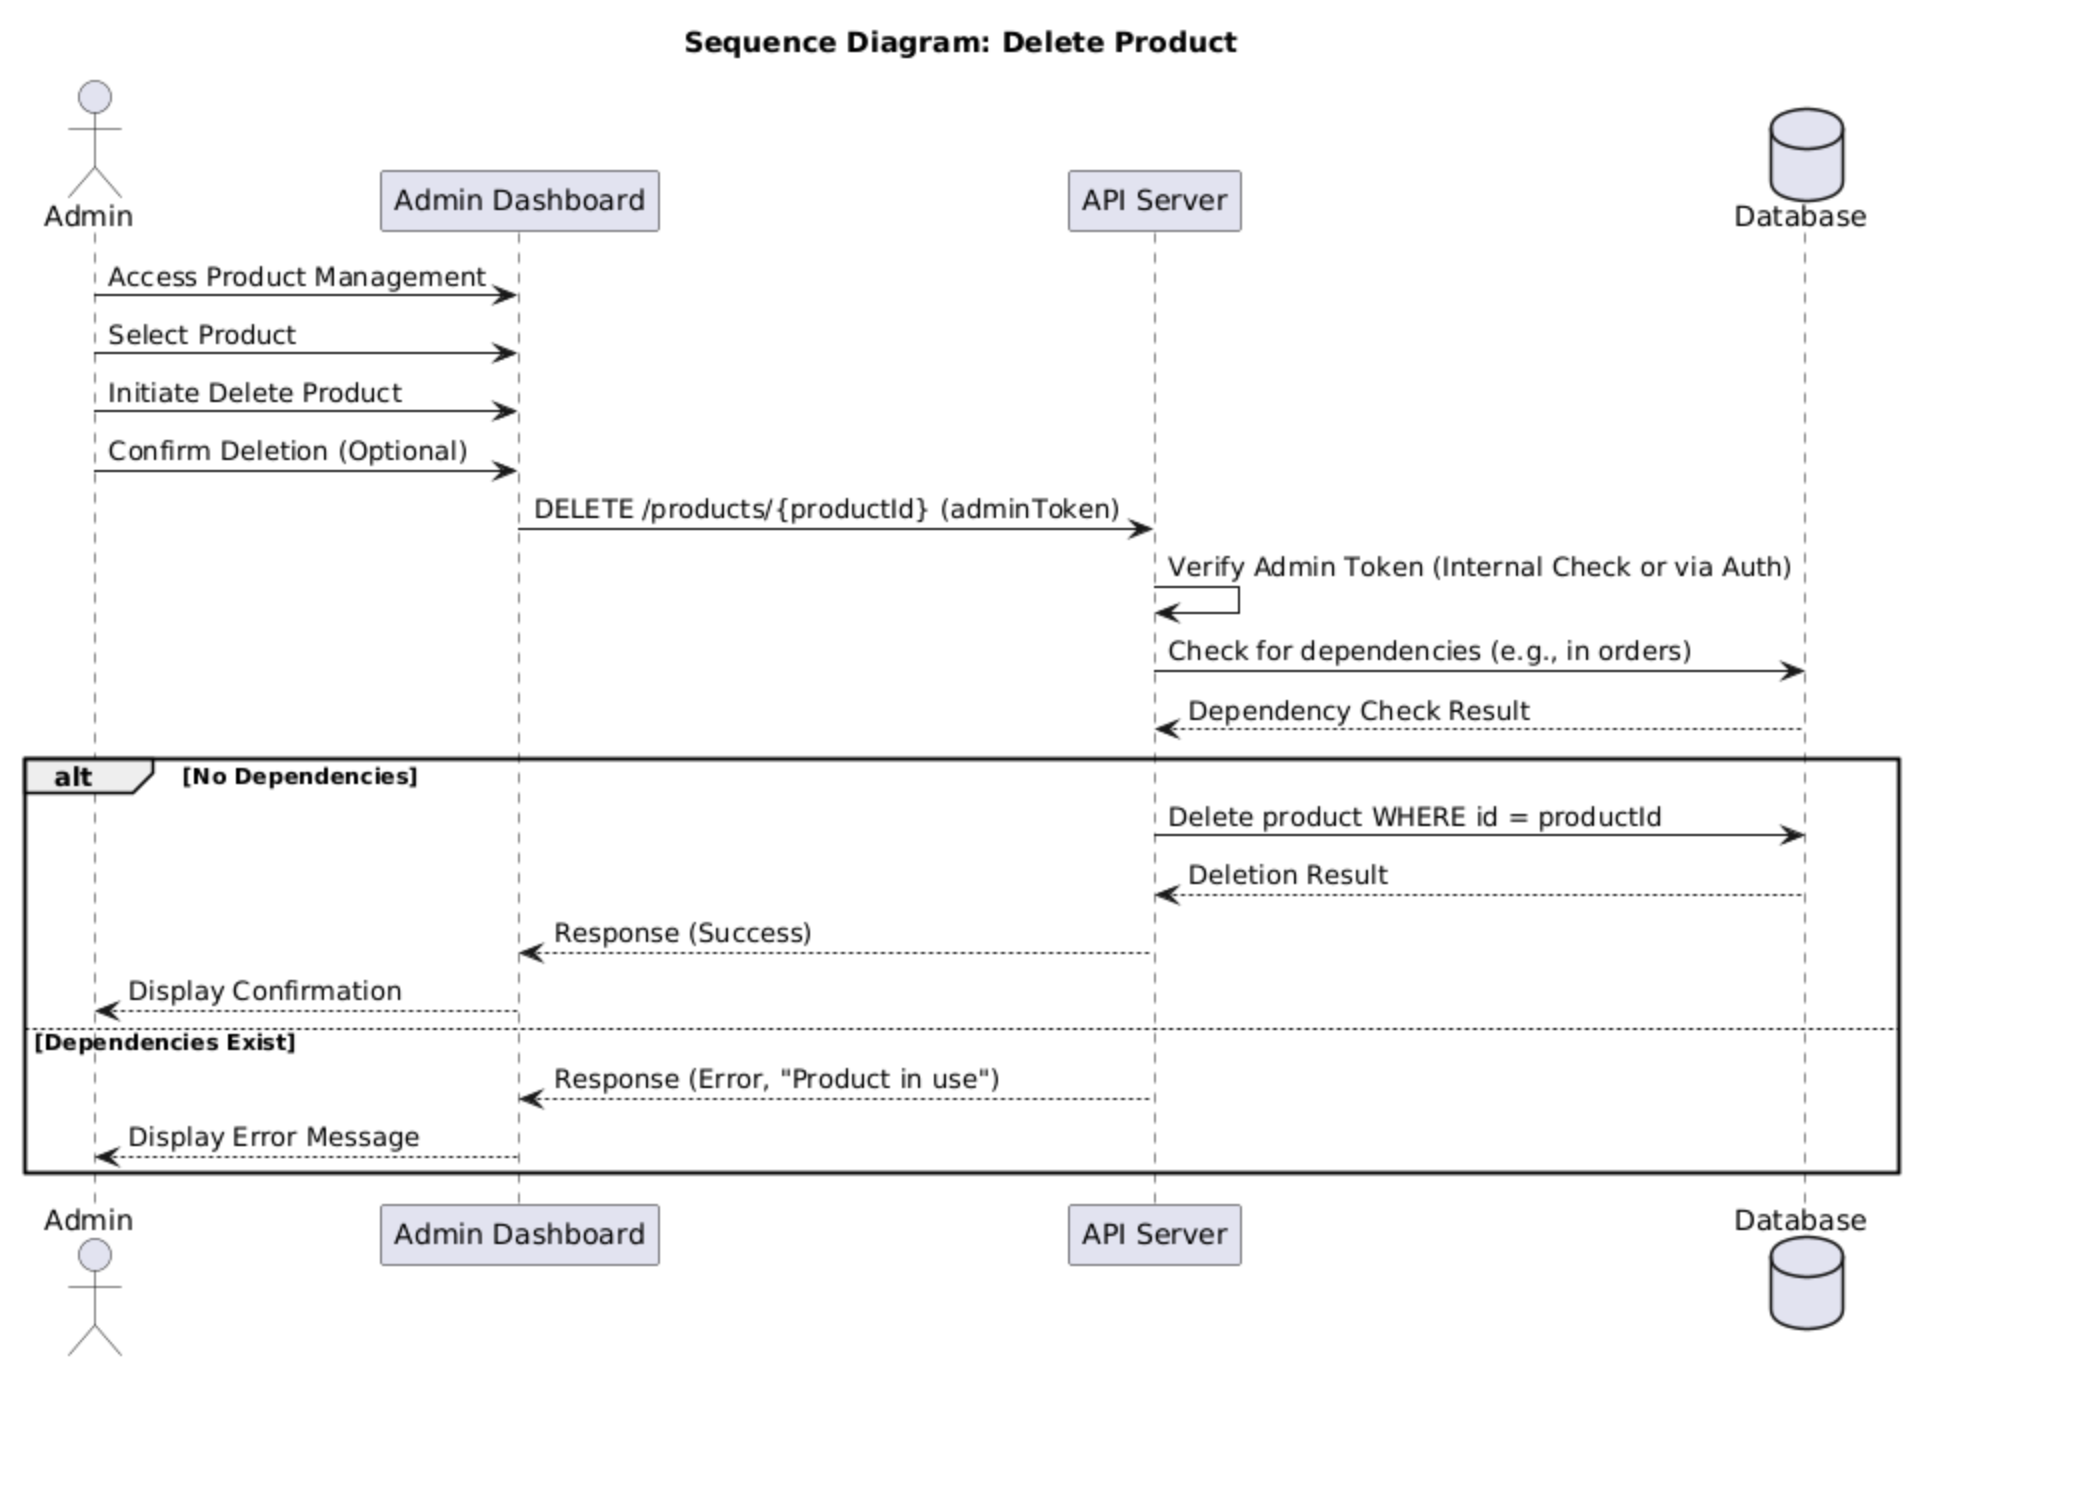
\includegraphics[width=0.9\textwidth]{figures/images/sprint2sequence(delete product).png}
  \caption{Sprint 2 – Delete Product Sequence Diagram}
  \label{fig:sprint2-delete-product}
\end{figure}

\section{API Endpoints for Admin Operations}

RESTful API endpoints were implemented to support admin functions:

\subsection*{User Management APIs}
\begin{itemize}
  \item \texttt{GET /api/admin/users} – Retrieve all users
  \item \texttt{POST /api/admin/users} – Create new user
  \item \texttt{PUT /api/admin/users/[id]} – Update user details
  \item \texttt{DELETE /api/admin/users/[id]} – Delete user account
\end{itemize}

\subsection*{Product Management APIs}
\begin{itemize}
  \item \texttt{GET /api/admin/products} – Retrieve product catalog
  \item \texttt{POST /api/admin/products} – Add new product
  \item \texttt{PUT /api/admin/products/[id]} – Update product
  \item \texttt{DELETE /api/admin/products/[id]} – Remove product
\end{itemize}

\section{Security and Validation}

\subsection*{Access Control}

Administrative functions are protected through:
\begin{itemize}
  \item Role-based access control (RBAC) verification
  \item JWT token validation for all admin endpoints
  \item Permission checks before sensitive operations
  \item Audit logging for administrative actions
\end{itemize}

\subsection*{Data Validation}

Input validation includes:
\begin{itemize}
  \item Email format validation for user accounts
  \item Product price and stock quantity validation
  \item Image upload size and format restrictions
  \item SQL injection prevention through parameterized queries
\end{itemize}

\section{Implementation Highlights}

\subsection*{Frontend Architecture}

The admin interface was built using:
\begin{itemize}
  \item React components with TypeScript for type safety
  \item Tailwind CSS for responsive design and consistent styling
  \item React Hook Form for efficient form management
  \item SWR for data fetching and caching
\end{itemize}

\subsection*{State Management}

Administrative data is managed through:
\begin{itemize}
  \item React Context for global admin state
  \item Local component state for form handling
  \item SWR cache for API data synchronization
  \item Optimistic updates for better user experience
\end{itemize}

\section{Testing and Quality Assurance}

Comprehensive testing was performed on:

\begin{itemize}
  \item User creation, modification, and deletion workflows
  \item Product CRUD operations and data integrity
  \item Role assignment and permission enforcement
  \item Stock level updates and inventory tracking
  \item Error handling and edge case scenarios
\end{itemize}

Manual testing verified that all administrative functions work correctly and securely, with proper validation and error messages displayed to users.

\section{Implementation Results}

The administrative interface was successfully implemented providing comprehensive management capabilities for system administrators.

% Admin Panel Screenshots
\begin{figure}[H]
  \centering
  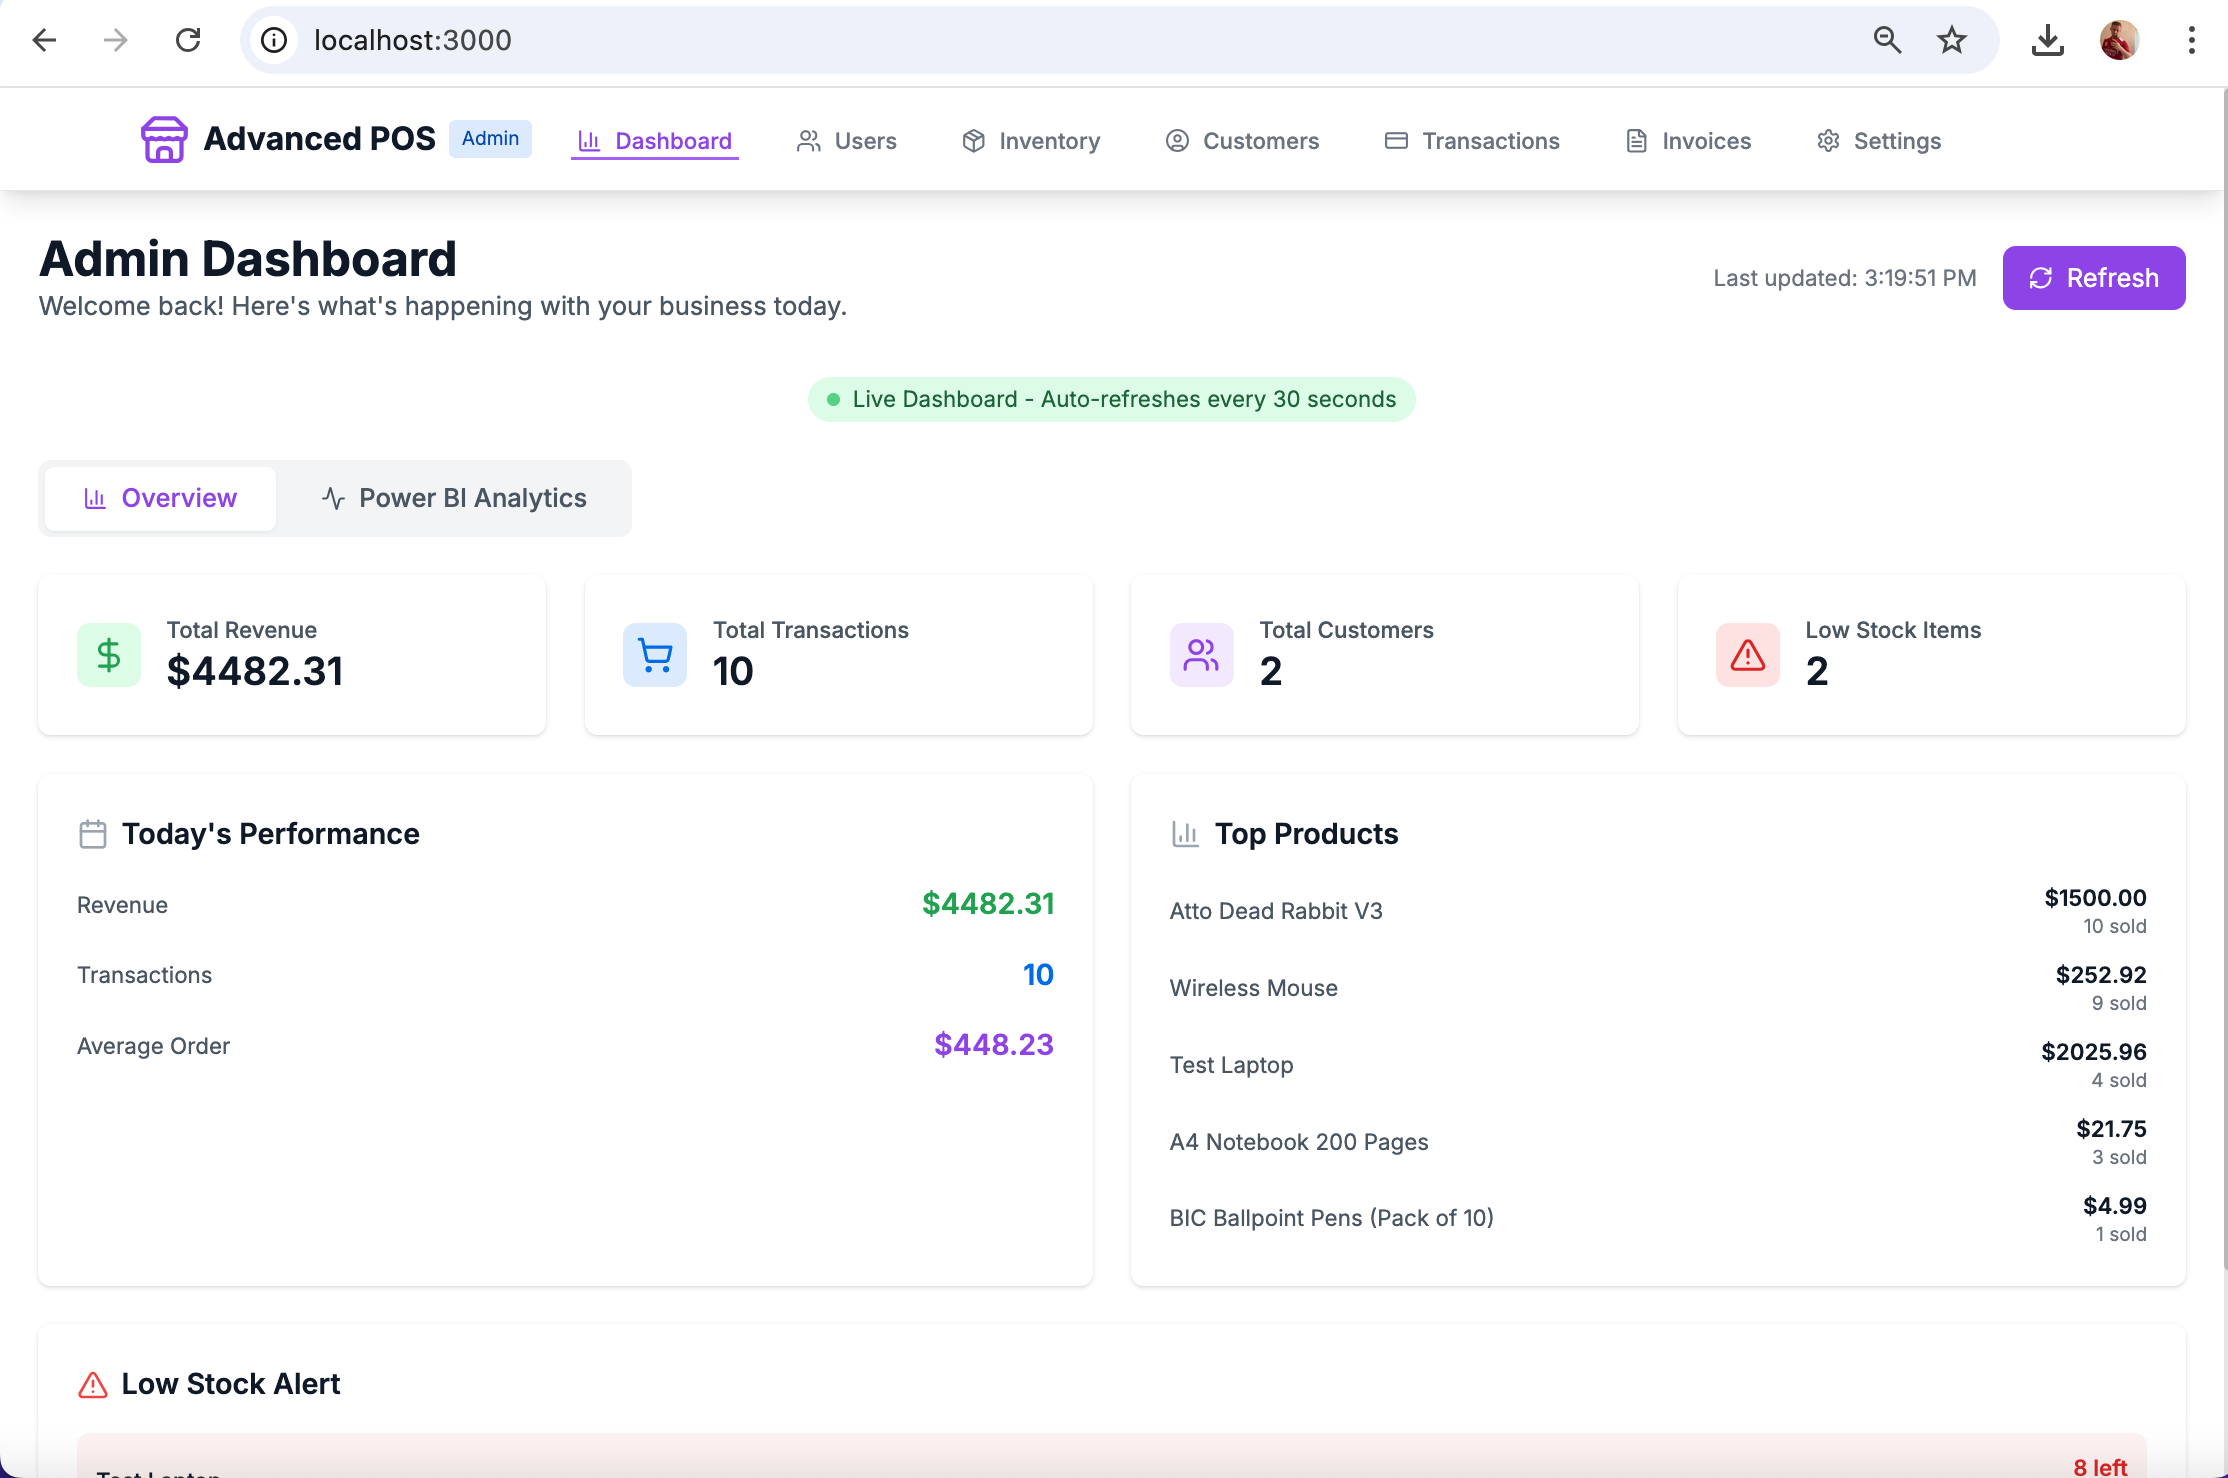
\includegraphics[width=0.9\textwidth]{working app screenshots/adminpanel.png}
  \caption{Admin Dashboard Overview - Central management interface with system metrics and navigation}
  \label{fig:adminpanel}
\end{figure}

\begin{figure}[H]
  \centering
  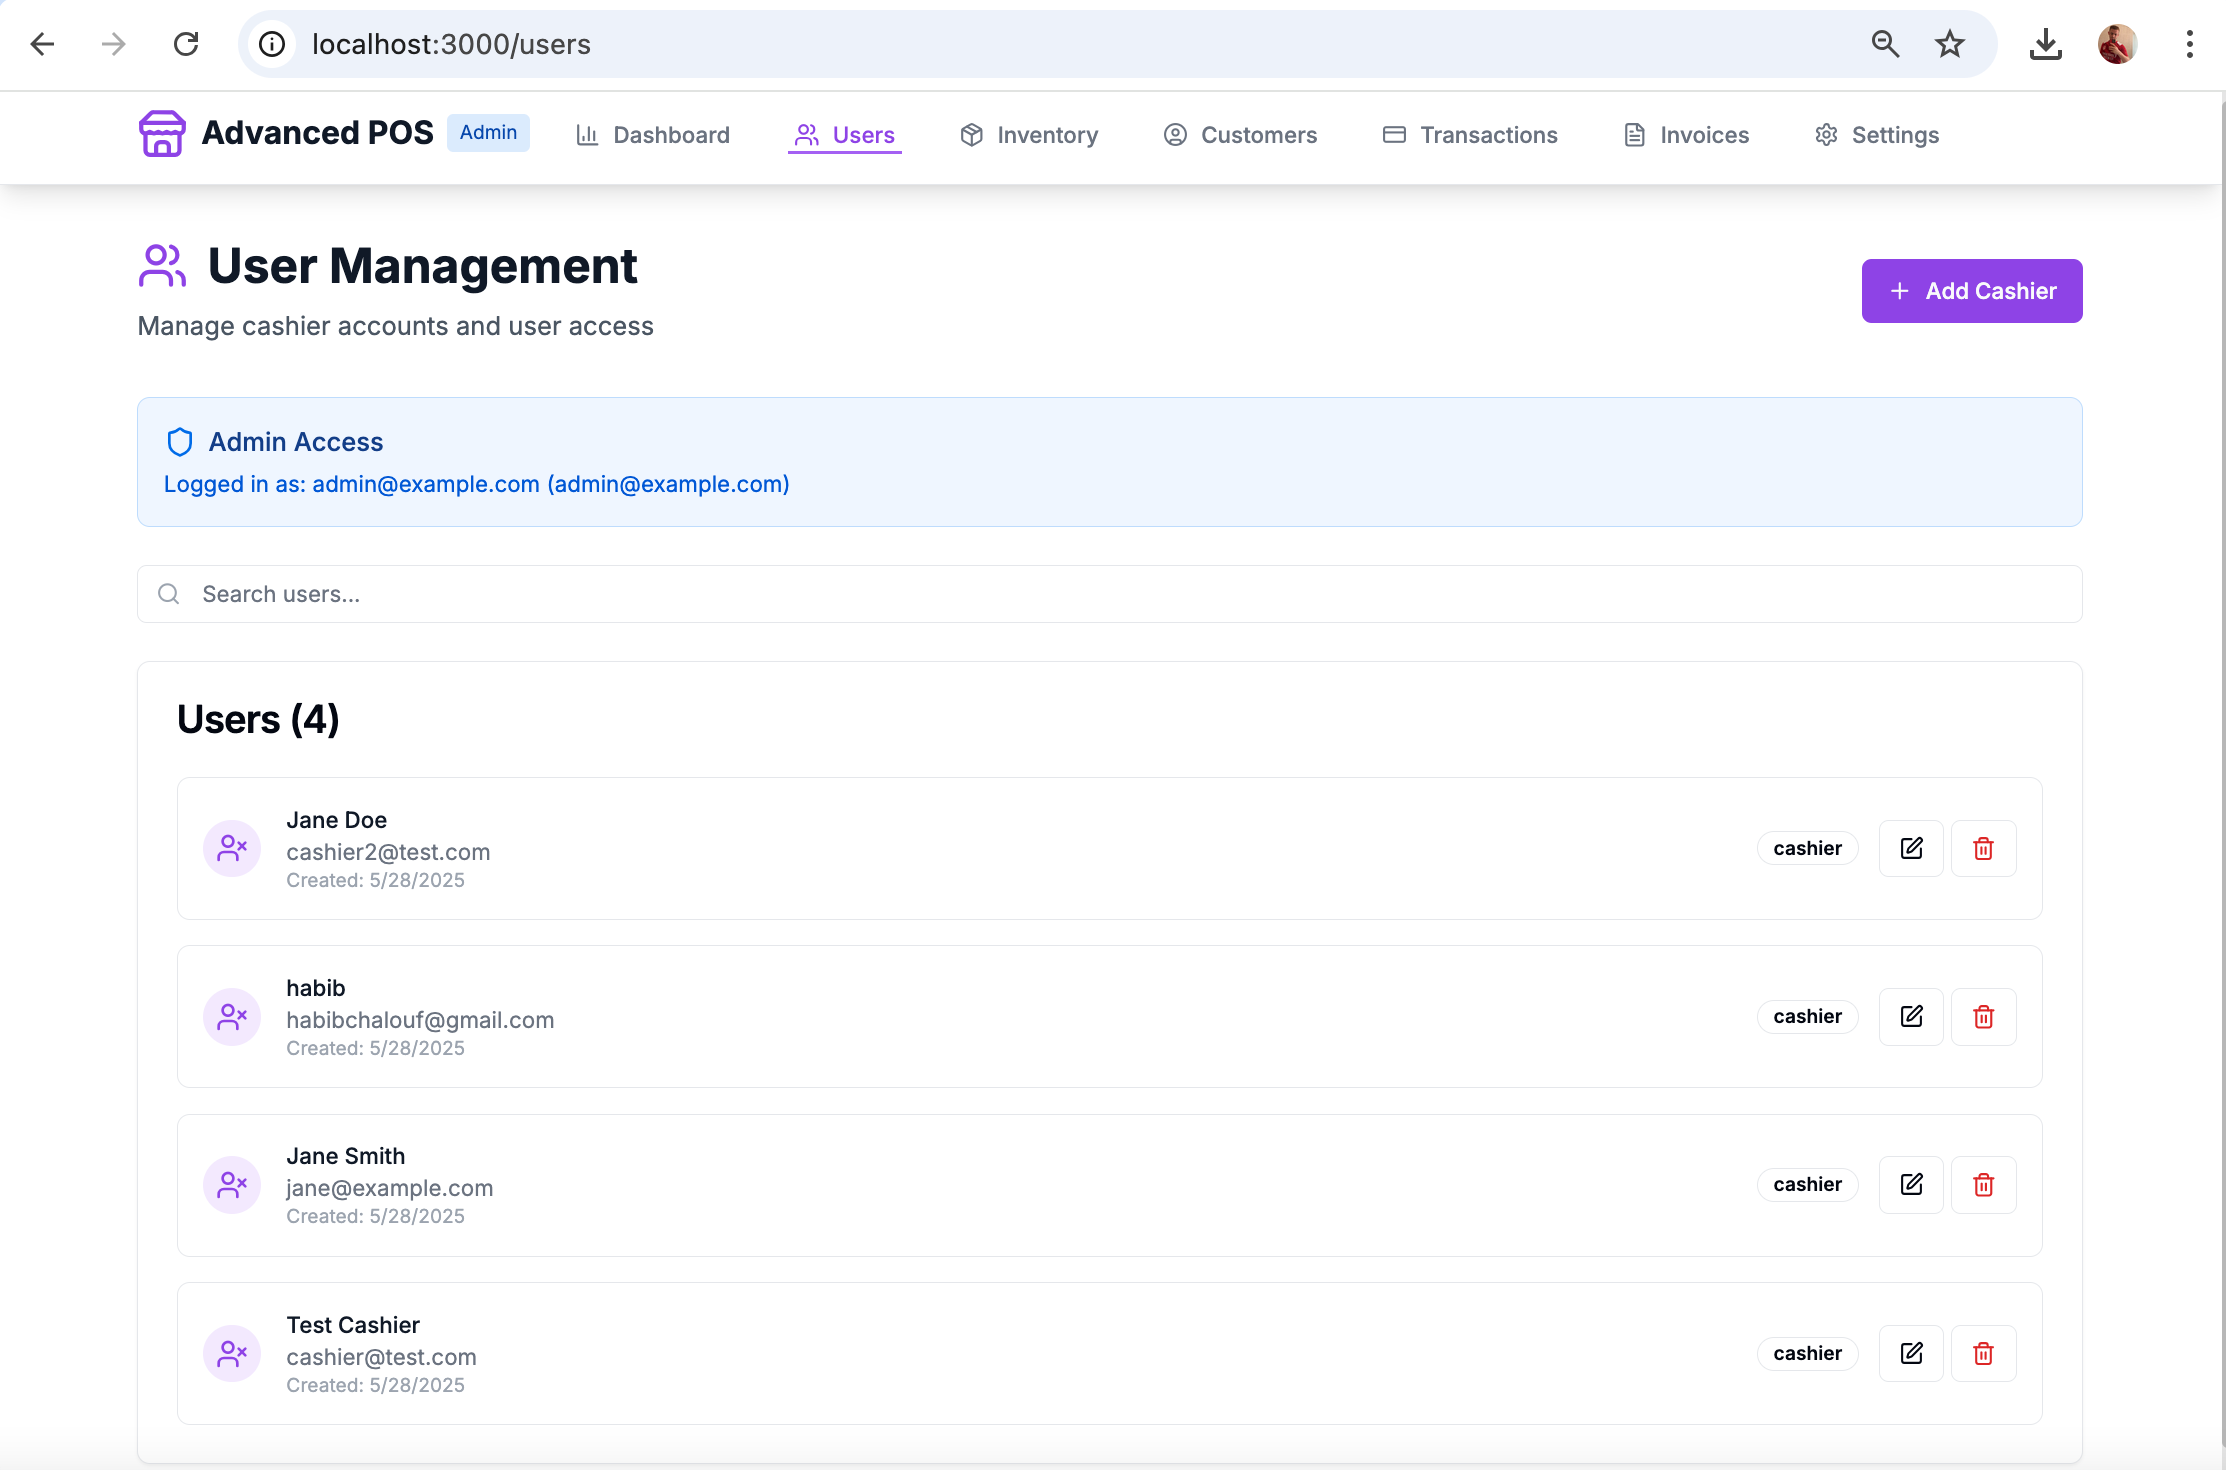
\includegraphics[width=0.9\textwidth]{working app screenshots/usermanagement.png}
  \caption{User Management Interface - CRUD operations for system users with role assignment}
  \label{fig:usermanagement}
\end{figure}

\begin{figure}[H]
  \centering
  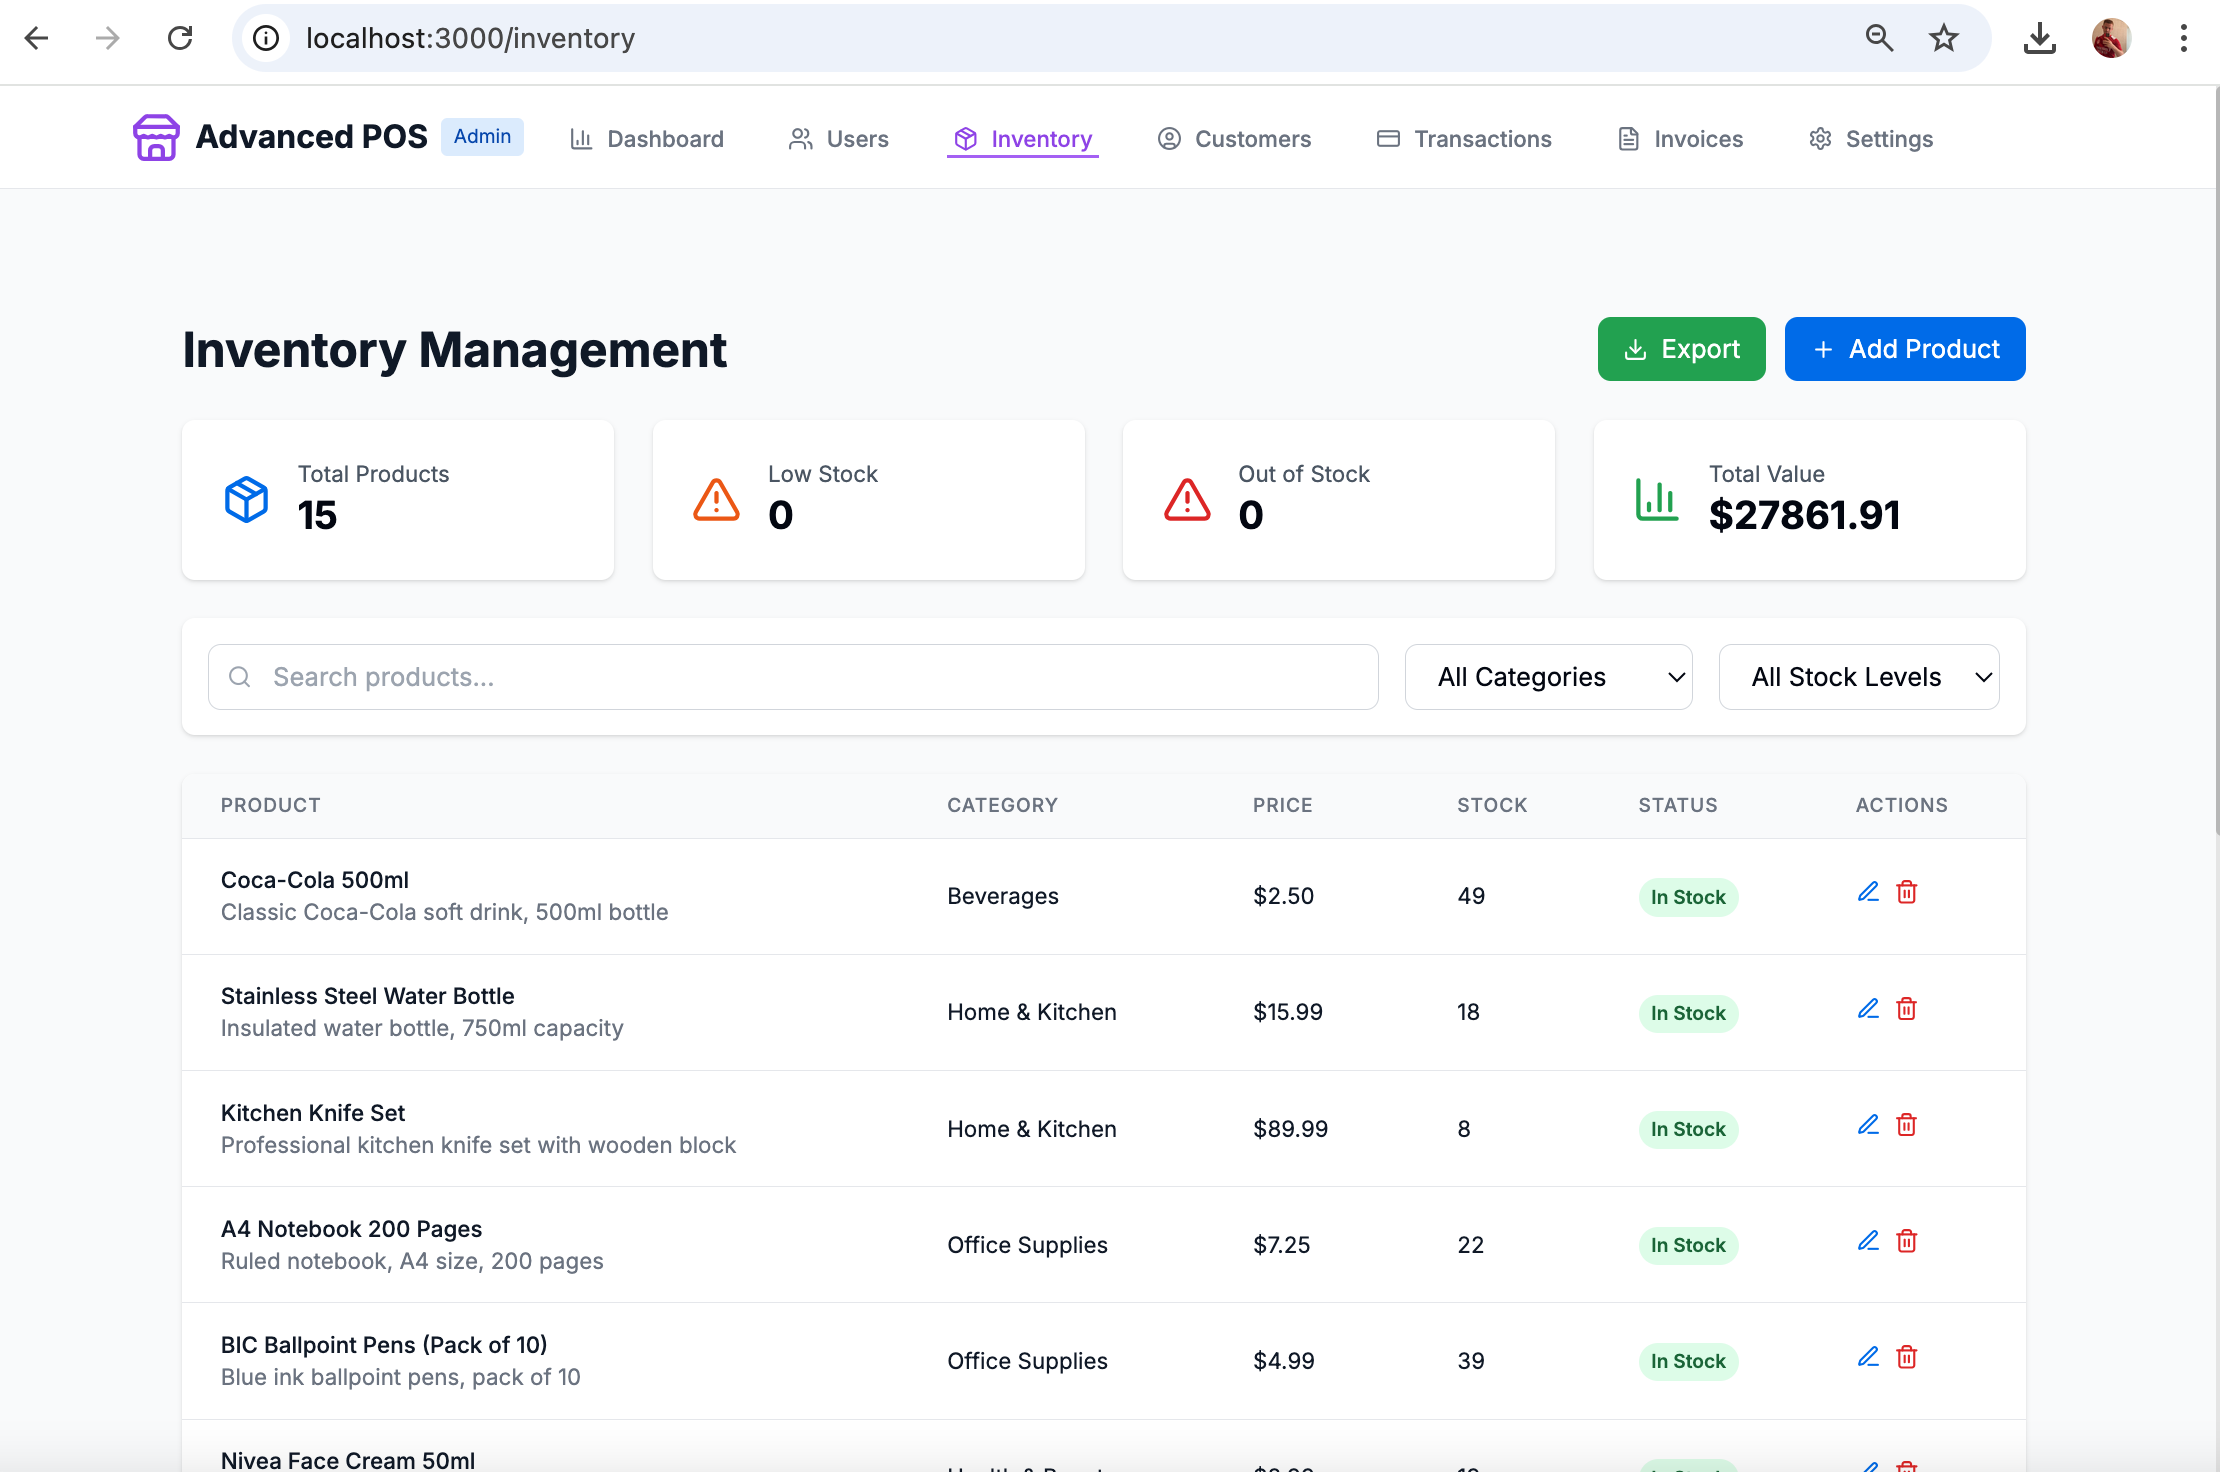
\includegraphics[width=0.9\textwidth]{working app screenshots/productmanagement.png}
  \caption{Product Management System - Inventory control with category management and stock tracking}
  \label{fig:productmanagement}
\end{figure}

\begin{figure}[H]
  \centering
  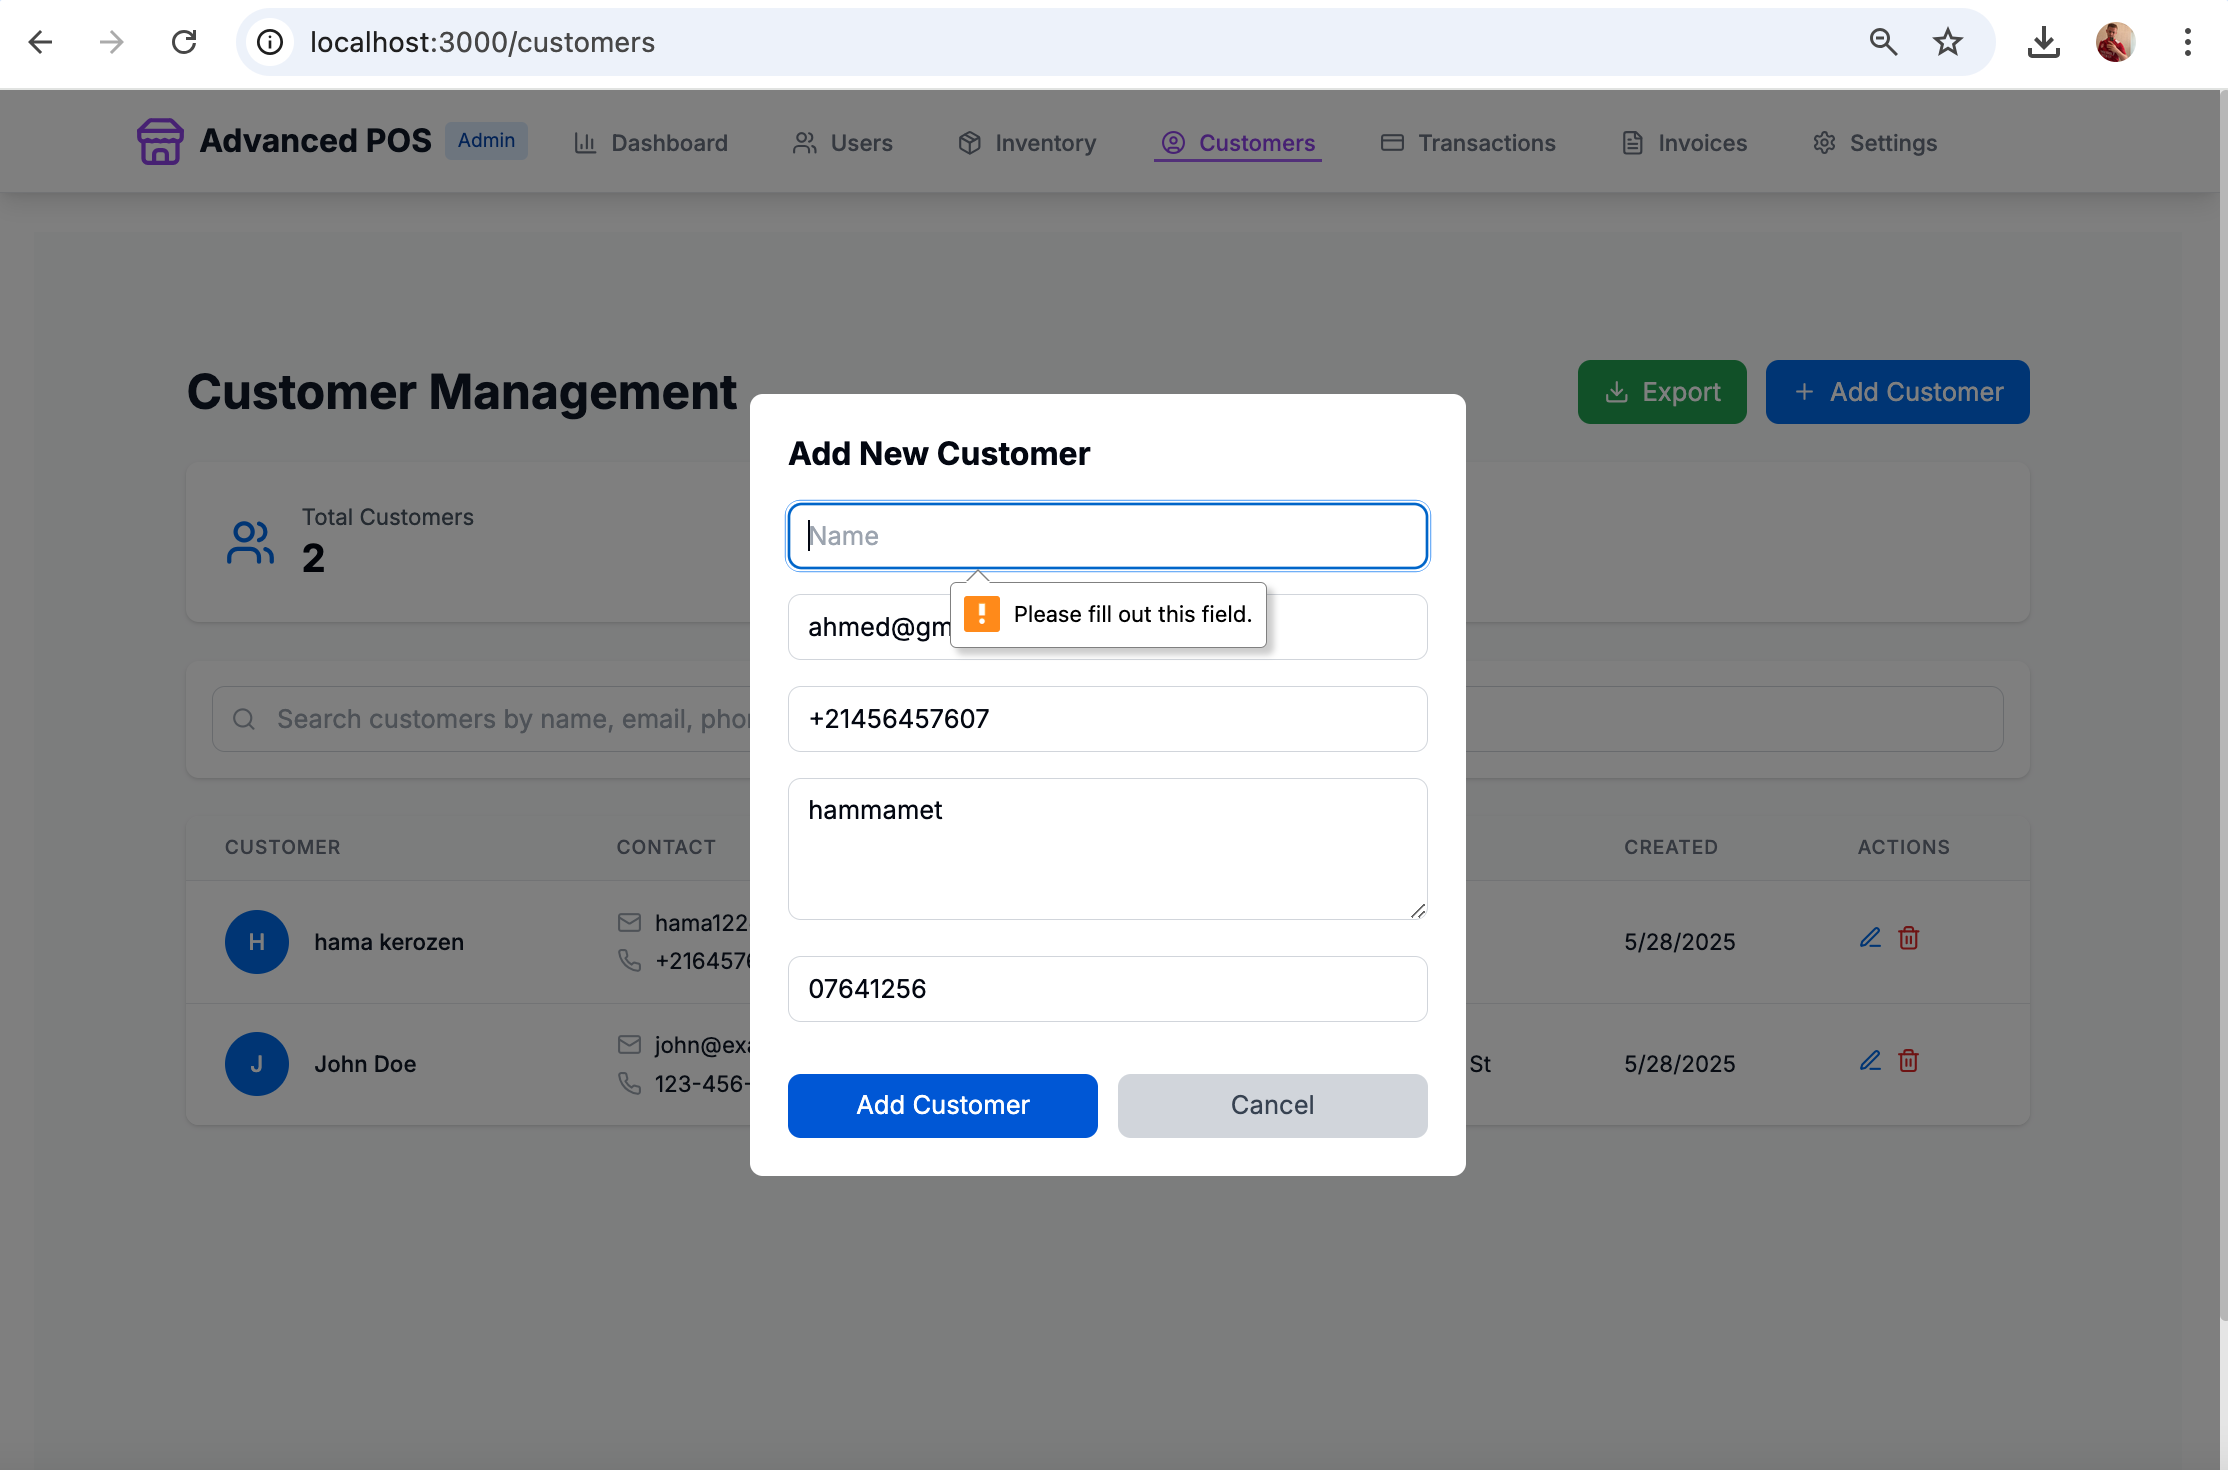
\includegraphics[width=0.9\textwidth]{working app screenshots/customererror.png}
  \caption{Form Validation Example - Error handling and user feedback for data integrity}
  \label{fig:customererror}
\end{figure}

The administrative system provides:

\begin{itemize}
  \item Comprehensive dashboard with key performance indicators and system health metrics
  \item Complete user management with role-based access control and permission assignment
  \item Full product lifecycle management including categories, pricing, and inventory tracking
  \item Robust form validation with clear error messaging and user guidance
  \item Responsive design ensuring optimal experience across different devices and screen sizes
\end{itemize}

\section{Conclusion}

Sprint 2 successfully delivered a comprehensive administrative interface that enables proper system management. Administrators can now effectively manage users, maintain the product catalog, and control inventory levels through an intuitive and secure interface. The next sprint will focus on building the POS interface for cashiers and implementing the invoicing system.
